\chapter{Graphs of Brownian motion}
\label{chap:graphs}

\section{Introduction}
\label{sec:intro-brownian}


Studying the dimension of various random processes has been of interest for quite some time, from \cite{taylor} to \cite{falconer-levy}. In this chapter we will consider the Assouad and lower dimensions of graphs of certain random processes, notably L\'evy processes and functions defined by stochastic integrals. Then the regularity dimensions of pushforward measures onto graphs of L\'evy processes will be computed for doubling measures defined on the unit interval. In particular we will see that pushforwards of doubling maps in this setting are almost surely \textit{not} doubling. This contrasts with the previous chapter's results on quasisymmetric homeomorphisms which conserved doubling; similarly for uniform perfectness. Furthermore, this will provide a nice example of a uniformly perfect and doubling space with a non uniformly perfect and non doubling measure fully supported on that same space.


\section{Graphs of L\'evy processes}
\label{sec:levy-process}


\emph{L\'{e}vy processes} $X(t)$ were first introduced by Paul L\'evy in 1934 \cite{levy} and are defined to be the stochastic processes satisfying:
\begin{itemize}
	\item[1]: $X(0)=0$ almost surely.
	\item[2]: For all $t,h>0$, $X(t+h)-X(t)$ is equal to $X(h)$ in distribution (stationary increments).
	\item[3]: For all $0<t_1<t_2<...<t_k$ the random variables $X(t_i)-X(t_{i-1})$ are independent (independence of increments).
	\item[4]: For all $t>0$ $\lim_{h\to 0} X(t+h)-X(t)=0$ in probability (continuity).
\end{itemize}

We can construct $X(t)$ such that it is almost surely right continuous with left limits (denoted c\`adl\`ag). Such processes are standard tools in many areas of modern mathematics and its applications. A common example of a L\'evy process is the \emph{Wiener process} (or Brownian motion) where property 2 (stationary increments) is replaced by Gaussian increments, so $X(t+h)-X(t)$ is normally distributed with mean 0 and variance $h$. One can similarly define $d$-dimensional Brownian motion by considering the vector-valued stochastic process $(W_1,\ldots, W_d)$ where the $W_i$ are independent Weiner processes. 


\begin{figure}[h]
    \centering
	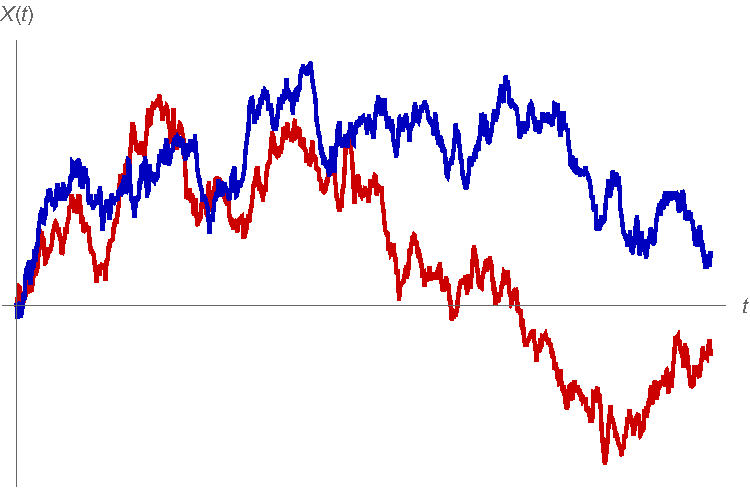
\includegraphics[width=0.5\textwidth]{pics/ch-brownian/wiener_process.pdf}
	\caption{\label{fig:brownianmotion}Two graphs of one-dimensional Brownian motion}
\end{figure}

The geometric properties, such as dimension, of Wiener processes have been a particularly well studied area. This includes studying the \emph{graphs}, \emph{level sets} and \emph{trails} of such processes which can be thought of as fractals as they often display some \emph{statistical self-affinity}. For any left continuous function $X:\mathbb{R}\to\mathbb{R}$, we define the graph of the function restricted to the interval $I \subseteq \mathbb{R}$ by
\nomenclature[G]{$G^{I}_{f}$}{graph of the function $f$ restricted to the interval $I$}
\[
G^{I}_{X}=\{(t,y) \colon \, y=X(t),t\in I\}\cup J,
\]
where $J$ is the union of vertical segments joining the discontinuities. $J$ is well defined because $X$ is right continuous. It is clear that if $X$ is continuous then $J$ is empty and as Wiener processes are almost surely continuous $J$ will not matter in this setting and can be safely ignored. This is not true for other L\'evy processes and so the $J$ are included for generality.

Taylor \cite{Ta} first calculated the Hausdorff dimension of $d$-dimensional Brownian motion $B_d:\mathbb{R}\to\mathbb{R}^d$ where he showed that almost surely
\[
\dim_\text{H} G_{B_1}^{[0,1]} = \dim_{\textup{B}}  G_{B_1}^{[0,1]} = \frac{3}{2}         
\]
and for any $d\ge 2$
\[
\dim_\text{H} B_d([0,1]) = \dim_{\textup{B}} B_d([0,1]) =  2.
\]


\begin{figure}[htbp]
	\centering
	\begin{subfigure}{0.3\textwidth}
		\centering
		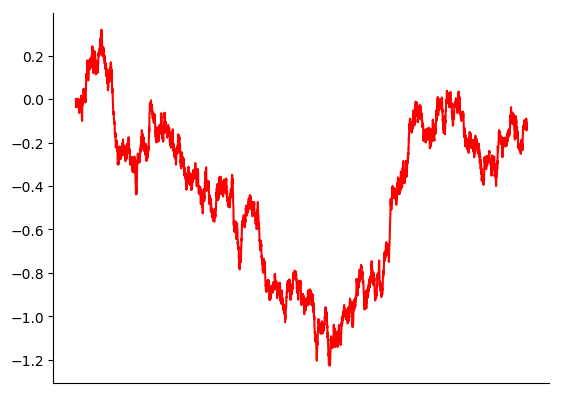
\includegraphics[width=0.85\linewidth]{pics/ch-brownian/2-brownianr.png}
	\end{subfigure}%
	\begin{subfigure}{.3\textwidth}
		\centering
		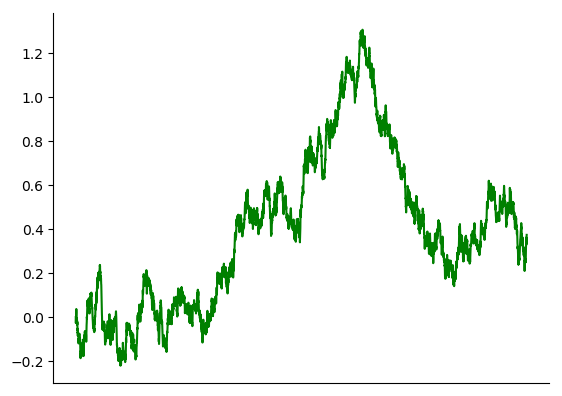
\includegraphics[width=.9\linewidth]{pics/ch-brownian/2-browniang.png}
	\end{subfigure}%
	\begin{subfigure}{.3\textwidth}
		\centering
		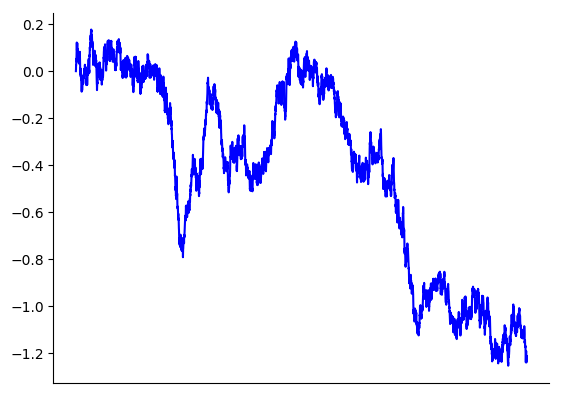
\includegraphics[width=.9\linewidth]{pics/ch-brownian/2-brownianb.png}
	\end{subfigure}
	\caption{Three graphs of Brownian motion, a 2-stable L\'evy process}
	\label{fig:brownian}
\end{figure}




One can formalise the aforementioned statistical self-affinity of L\'evy process. However, not all processes have this property so we will restrict to what are called \textit{stable} or $\alpha$-\textit{stable processes}, that is where, for some $\alpha > 0$,
\[
c^{-1/\alpha}X(ct) =^d X(t)
\]
for all $c,t > 0$ and $=^d$ means equal in distribution. Two such random variables $X,Y$ are equal in distribution if $P(X \le t) = P(Y \le t)$ for all $t \in \mathbb{R}$.  We will sometimes refer to $\alpha$ as the scaling coefficient of $X$. It has been shown that such $\alpha$-stable L\'evy processes have
\[
\dim_\text{H} G_{X_1}^{[0,1]} = \dim_{\textup{B}}  G_{X_1}^{[0,1]} = \max\{1, 2 - 1/\alpha\},
\]
recovering the Brownian motion result above by setting $\alpha = 2$. Note that when $\alpha < 1$ then the graph simply has Hausdorff dimension one with full probability, the lowest possible dimension, as these processes are constant except between certain jump discontinuities. In particular the frequency of these jumps is low enough to not raise this dimension.

Our final condition for these processes is a simple assumption that the distribution $X(1)$ is non-vanishing on $\mathbb{R}$. Non-zero on an interval would also work, this is just to ensure the graphs are not just multiple flat lines, such as in a Poisson process. This ensures genuinely interesting geometric behaviour.

\begin{figure}[htbp]
	\centering
	\begin{subfigure}{0.3\textwidth}
		\centering
		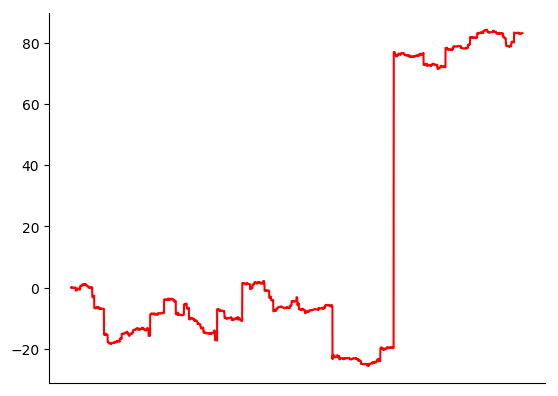
\includegraphics[width=0.85\linewidth]{pics/ch-brownian/1-cauchyr.png}
	\end{subfigure}%
	\begin{subfigure}{.3\textwidth}
		\centering
		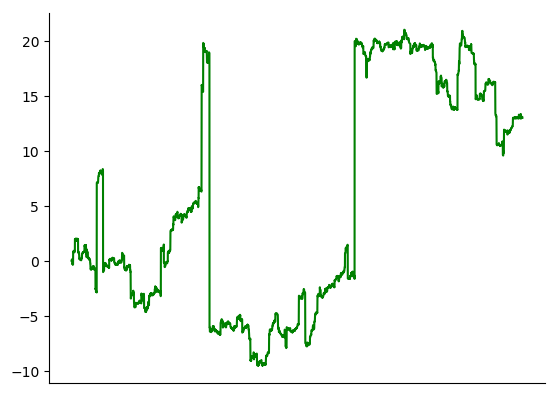
\includegraphics[width=.9\linewidth]{pics/ch-brownian/1-cauchyg.png}
	\end{subfigure}%
	\begin{subfigure}{.3\textwidth}
		\centering
		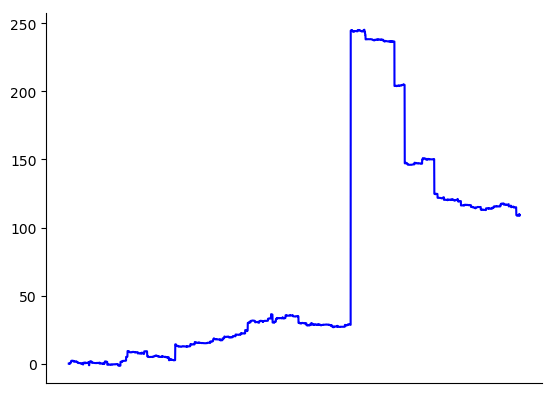
\includegraphics[width=.9\linewidth]{pics/ch-brownian/1-cauchyb.png}
	\end{subfigure}
	\caption{Three graphs of a L\'evy process whose increments are Cauchy distributed, a 1-stable L\'evy process}
	\label{fig:cauchy}
\end{figure}

Another generalisation of Brownian motion is \emph{fractional Brownian motion}, first introduced by Mandelbrot and van Ness \cite{MVN}. Index-$h$ fractional Brownian motion (fBm) on $\mathbb{R}$ with $0<h<1$ is defined to be the stochastic integral 
\[
B_h (t) = c(h)^{-1} \int_{-\infty}^\infty \left(\left( t-x \right)_+^{h-1/2} - (-x)_+^{h-1/2} \right)dW(x)
\]
where the integral is an It\^{o} integral with respect to the Wiener process, $(x)_+ = \max\{0,x\}$ and $c(h) = \Gamma(h+1/2)$, where $\Gamma$ denotes the gamma function. Many standard books on stochastic calculus will introduce the It\^{o} intergral, we will later refer to \cite{protter} for further properties of this intergal. Equivalently this is a Gaussian random process $B_h(t)$ with:
\begin{itemize}
	\item[1]: $B_h(0)=0$ almost surely.
	\item[2]: For all $t,u>0$, $B_h(t+u)-B_h(t)$ has normal distribution with mean 0 and variance $u^{2h}$ (Gaussian increments).
	\item[3]: For all $t>0$, $\lim_{u\to 0} B_h(t+u)-B_h(t)=0$ in probability (continuity).
\end{itemize}
One can see that when $h=1/2$, $B_{1/2}(t) = B(t)$ is simply Brownian motion. Several equivalent definitions for fBm exist, we choose to use the It\^{o} integral form as our results follow more directly in this setting. Note that fractional Brownian motion is not a L\'evy process as its increments are not independent, except when $h = 1/2$ where we recover regular Brownian motion. Much progress has been made on the properties of fBm, see for instance \cite{Ad},\cite{Ka} and \cite{Fa2}. Notably it was shown that almost surely, the graph over the unit interval of index-$h$ fBm has Hausdorff dimension $2-h$. 

\begin{figure}[h]
	\centering
	\begin{subfigure}[b]{0.3\textwidth}
		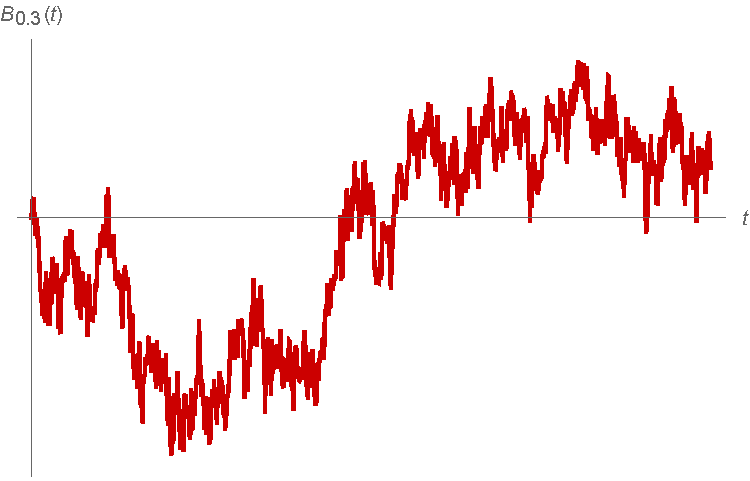
\includegraphics[width=\textwidth]{pics/ch-brownian/fbm0_3.pdf}
		\caption{Graph of fBm with h=0.3}
		\label{fig:fbm3}
	\end{subfigure}
	~ %add desired spacing between images, e. g. ~, \quad, \qquad, \hfill etc. 
	%(or a blank line to force the subfigure onto a new line)
	\begin{subfigure}[b]{0.3\textwidth}
		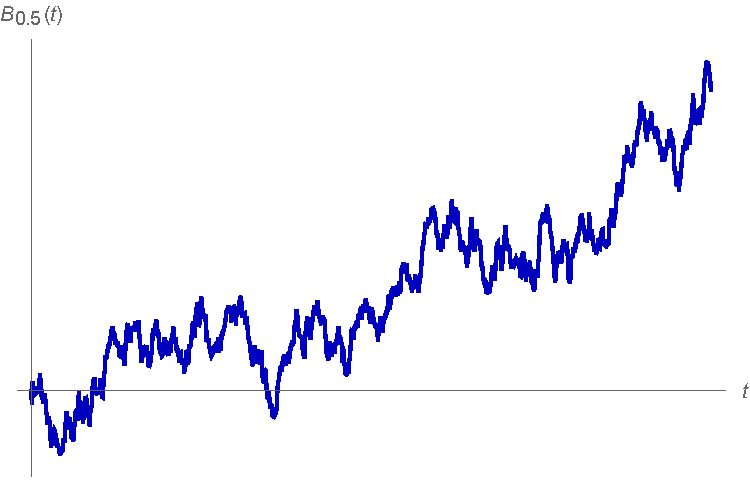
\includegraphics[width=\textwidth]{pics/ch-brownian/fbm0_5.pdf}
		\caption{Graph of fBm with h=0.5}
		\label{fig:fbm5}
	\end{subfigure}
	~ %add desired spacing between images, e. g. ~, \quad, \qquad, \hfill etc. 
	%(or a blank line to force the subfigure onto a new line)
	\begin{subfigure}[b]{0.3\textwidth}
		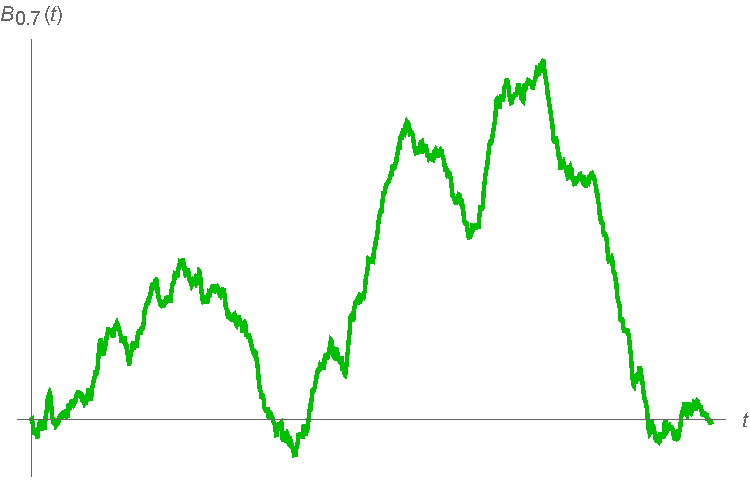
\includegraphics[width=\textwidth]{pics/ch-brownian/fbm0_7.pdf}
		\caption{Graph of fBm with h=0.7}
		\label{fig:fbm7}
	\end{subfigure}
\end{figure}


Studying the Assouad dimension of various fractals and its properties is an increasingly popular area of research. It is therefore natural to calculate the Assouad dimension of the graph $G_X^{[0,1]}$ for $\alpha$-stable L\'{e}vy processes and stochastic integrals $X$. As the Assouad dimension provides information on the extremal local scaling of a set, in this setting it will tell us about the maximal fluctuations of a random process and so we expect the dimension to be full. Similarly for the lower dimension, we expect it to pick up on the sparsest behaviour; in this case the lower dimension should treat the graph as if it were a smooth line.


\begin{theorem}\label{Main}
	Let $X$ be an $\alpha$-stable L\'evy process with $\alpha \geq 1$ such that $X(1)$ is a random variable whose distribution function is non-vanishing almost everywhere. Then almost surely
	\[
	\Assouad G_{X}^{[0,1]} = 2
	\]
	and 
	\[ 
	\lowerdim G_{X}^{[0,1]} = 1.
	\]
\end{theorem}

Interestingly the Assouad and lower dimensions of the graph do not depend on the scaling coefficient, unlike the Hausdorff dimension. However we do not obtain a formula for $\alpha \in (0,1)$ for the Assouad dimension as our technique does not extend to this setting; it is possible that with such a parameter, the Assouad dimension would decrease to one as a function of $\alpha$. But it is also possible that the Assouad dimension of these graphs is simply one, as the distribution of a jump discontinuity of height greater than $R$ in an interval of width $r$ is Poisson with mean $r/R^\alpha$. Further study of this question could result in a novel answer.

\begin{question}
For any $\alpha \in (0,1)$, it is known that the graph of an $\alpha-$stable L\'evy process almost surely has dimension 1 for many notions of dimension. What is the Assouad dimension of these graphs?
\end{question}


A particular case of this theorem is, as the Wiener process $W(t)$ is a $2$-stable L\'evy process, the following.
\begin{corollary}
Almost surely
	\[
	\Assouad G_{W}^{[0,1]}=2
	\]
	and 
	\[
	\lowerdim G_{W}^{[0,1]}=1.
	\]
\end{corollary}

Brownian motion also provides examples of Salem sets that can have different Hausdorff and Assouad dimensions, we refer the reader to \cite{Ka}  for further discussion on the links between random processes and Salem sets.

Ville Suomala and Changhao Chen, in a personal communication, kindly remarked that the Assouad part of this corollary follows from the graph of Brownian motion having full lower porosity dimension. This approach is inspired by \cite{coxgriffin}, where it was shown that the graph of Brownian motion has full upper porosity dimension. However this porosity dimension technique does not extend to our following, more general result.

We can say more about the Assouad dimension of random processes which are functions defined as stochastic integrals. 

\begin{theorem}\label{ch-brownian:stochastic}
	Let $f:\mathbb{R}\to\mathbb{R}$ be a function which is zero only finitely often and is $C^2$ on some interval. Then we define $B_f(t)$ as the function defined by the stochastic integral
	\[	
	B_f(t)=\int_0^t f(x) dW(x).
	\]
	We have that almost surely:
	\[
	\Assouad G_{B_f}^{[0,1]}=2.
	\]
\end{theorem}

In particular, graphs of fractional Brownian motions with indices $0<h<1$ have full Assouad dimension almost surely. The conditions in this theorem are designed to ensure $f$ is a reasonably smooth, non-zero function which will allow the random Wiener process to dictate the behaviour of the graph. Usually these integrals are with respect to a random function, but controlling the interaction between a random function and the Wiener process raises issues in this setting and so is left as an open problem. 

\begin{question}
Can a lower dimension analogue of Theorem \ref{ch-brownian:stochastic} be found? Given that this result mirrors the Assouad dimension of the graphs of Brownian motion it is natural to conjecture that the lower dimension in this setting will be almost surely 1.
\end{question}


The proof of Theorem \ref{Main} can also be extended to higher dimensions. Thus one could show the following result.

Let $B_d(t)$ be the $d$-dimensional Brownian motion, from $\mathbb{R}$ to $\mathbb{R}^d$. Then almost surely
\[
\Assouad B_d([0,1])=d
\]
and 
\[
\lowerdim B_d([0,1]) = 1.
\]
	
We can compare this result to the well known \[\dim_{\mathrm{H}} B_d([0,1])=2\] for $d\geq 2$. The Hausdorff dimension being 2 here can be thought as a reflection that higher dimensional Brownian motion is transient, that is almost surely the process will diverge to infinity without returning to a neighbourhood infinitely often, whilst the Assouad dimension shows that there are still areas of maximal fluctuation. 



\section{Proofs regarding the dimensions of graphs}

This section will be dedicated to the proofs of Theorems \ref{Main} and \ref{ch-brownian:stochastic}. Section \ref{ch-brownian:sec:higher-dim} will provide an outline of a proof for the higher dimensional analogue of Theorem \ref{Main}.


\subsection{Assouad and lower dimensions of graphs}\label{ch:brownian:graph-proof}
In this section we will state a convenient condition to check whether a graph of a function $f:[0,1]\to\mathbb{R}$ has full Assouad dimension or lower dimension one. This will be leveraged in the following sections by showing graphs of different random processes satisfy the conditions stated here.


Let $R_1,R_2>0$ be positive numbers and $n>0$ be an integer. Given a point $a\in\mathbb{R}$, we define $W_{n}^{R_1\times R_2}((a, f(a)))$ as the following collection of sets
\begin{align*}
	\Bigg\{\left[a+\frac{i}{n}R_{1}, a+\frac{i+1}{n}R_{1}\right]\times \bigg[f(a)+\frac{j}{n}R_{2}&,f(a)+\frac{j+1}{n}R_{2}\bigg] \colon \\
	    & i,j\in\{0,\dots,n-1\}\Bigg\}.
\end{align*}
We see that $W_{n}^{R_1\times R_2}((a,f(a)))$ is the collection of rectangles of side lengths $R_1/n$ by $R_2/n$ and with disjoint interiors, which partitions the $R_1$ by $R_2$ rectangle of lower left vertex $(a,f(a))$.
	
Then let $N_{n}^{R_1 \times R_2 }((a,f(a)),G_f^{[0,1]})= \# \left\{ W_{n}^{R_1\times R_2}((a,f(a))) \cap G_f^{[0,1]} \right\}$, where $\#$ is the cardinality of the set, this provides the number of rectangles which intersect the graph.


The following proposition follows directly from the definition of Assouad dimension and the proof simply relies on noticing the relation between \newline$N_{n_1}^{R_1 \times R_1 }((a,f(a)),G_f^{[0,1]})$ and the covering number of an associated ball.


\begin{proposition}\label{graph}
	If there exists a constant $C>0$ and sequences:
	\[
	a_i\in \mathbb{R},R_i\in (0,1),\, n_i\in\mathbb{N} \quad (\forall i\in \mathbb{N})
	\]
	with $n_i \rightarrow \infty$ such that for all $i\in\mathbb{N}$
	\[
	N_{n_i}^{R_i \times R_i }((a_i,f(a_i)),G_f^{[0,1]})\geq C n_i^2.
	\]
	Then
	\[
	\Assouad G_f^{[0,1]}=2.
	\]
\end{proposition}

Whilst this might seem like a restrictive condition to ask a general function to satisfy, it is quite natural in the setting of L\'evy processes due to the almost sure unbounded variation and stable property of the process. Considering squares instead of balls in the definition of Assouad dimension is similar to the definition of the Furstenberg star dimension, which is in fact equivalent to the Assouad dimension, see \cite{chenwuwu}.

Note that one could replace the inequality $N_{n_i}^{R_i \times R_i }((a_i,f(a_i)),G_f^{[0,1]})\geq C n_i^2$ with the following equality
\[
N_{n}^{R_i \times R_i }((a_i,f(a_i)),G_f^{[0,1]})= n_i^2.
\]
This follows from \cite[Theorem 2.4]{FY}, where it is shown that a set has full Assouad dimension if and only if it has the unit ball as a weak tangent. This means that any cover of our set is also a cover of a ball and so all smaller squares are needed in the cover. This fact should be clear at the end of the proof in the next section but we leave the inequality in the proposition as it is easier to see the relation with the Assouad dimension in this form.


A similar statement can be made about the lower dimension and again, the proof relies on observing the relation between covering numbers of squares and balls. It is perhaps worth noting that even though the lower dimension is not monotone, as long as the function $f$ is c\`adl\`ag then the dimension of the graph with adjoining lines $J$ must be bounded below by 1.
\begin{proposition}\label{graph-lower}
	If there exists a constant $C'>0$ and sequences:
	\[
	a_i\in \mathbb{R},R_i\in (0,1),\, n_i\in\mathbb{N} \quad (\forall i\in \mathbb{N})
	\]
	with $n_i \rightarrow \infty$ such that for all $i\in\mathbb{N}$
	\[
	N_{n_i}^{R_i \times R_i }((a_i,f(a_i)),G_f^{[0,1]})\leq C' n_i
	\]
	and the intersection $W_n^{R_i \times R_i}((a_i,f(a_i))) \cap G_f^{[0,1]}$ includes at least all of the squares in the column 
	\begin{align*}
	    	\bigg\{ \left[a_i + \frac{j}{n_i}R_i, a_i + \frac{j+1}{n_i}R_i \right] &\times \left[f(a_i) + \frac{k}{n_i}R_i, f(a_i) + \frac{k+1}{n_i}R_i \right] \colon \\
	    	&j = \frac{\lfloor n_i/2 \rfloor }{n_i} \textup{ and } k = 0, 1,\ldots, n_i - 1 \bigg\}.
	\end{align*}
	Then
	\[
	\lowerdim G_f^{[0,1]}=1.
	\]
\end{proposition}

Here $\lfloor \cdot \rfloor$ is the floor function. When $n_i$ is odd the chosen column is clearly the centre of the square, when $n_i$ is even we simply take the column to the left of centre. In Proposition \ref{graph} we pass from the squares considered to balls of same centre and radius and as we are just trying to find a lower bound to the covering number, it suffices to cover one quarter of the ball, which is given by the cover of the square. For the lower dimension the goal is to obtain an upper bound so the entire ball must be understood, thus we must study a ball centred inside the square given by the assumptions. This leads us to ask for intersection in a centred column to guarantee the existence of a point which can be taken as the centre of a ball. The new condition in the above proposition stems from this technical point but could be weakened easily; this form suffices for our proof in the next section.

As with the Assouad dimension, the inequality $N_{n_i}^{R_i \times R_i }((a_i,f(a_i)),G_f^{[0,1]})\leq C' n_i$ will actually be an equality in the proof however this is not guaranteed as it was above. In \cite{microsets} it was show that a set has zero lower dimension if and only if it has a singleton as a weak tangent but this does not directly imply that a set of lower dimension one must have an interval as a weak tangent. In fact there exist examples of self-similar sets of dimension one with no interval as weak tangents. Whilst a somewhat artificial argument, this behaviour is expected to be the norm.


\subsection{Graphs of L\'evy processes}\label{LP}

Let $X(t)$ be an $\alpha$-stable L\'evy process with $\alpha \ge 1$. We assume that $X(1)$ is non-vanishing almost everywhere on $\mathbb{R}$ as a random variable, that is, the distribution function of $X(1)$ is 0 only on a set of zero measure. We start by proving the Assouad dimension result, the lower version will be a simple modification. This proof will aim to construct infinitely many events of positive probability such that the sum of their probabilities is infinite. Then, by Borel-Cantelli, infinitely many of these events must happen. If we have constructed the events correctly this will provide a sequence of rectangles which satisfy Proposition \ref{graph}, completing the proof.

The events we will consider will effectively be of the form `$N_{n}^{1 \times 1 }((0,0),G_X^{[0,1]})=n^2$' for some $n\in \mathbb{N}$, that is when the graph intersects all parts of the unit square. The probability of such an event can be computed and is a strictly positive number depending only on $n$; we denote this number by $P(n)$. The event `$X$ hits a rectangle' is measurable when $X$ is continuous; when it is discontinuous we join the graph with a vertical line and the process is c\`adl\`ag so the event `$X$ hits a rectangle' is still measurable. Thus our event is measurable as the union of measurable events. 

Denote $D(j)=[j/n,(j+1)/n]$ for all $j\in\{0,\dots, n-1\}$ then we can see that
\[
P(n)\geq P\left(\forall \, k\in\left[1,n^2\right], k\in \mathbb{N},X\left(\frac{k}{n^2}\right)\in D\left(\left\{\frac{k}{n}\right\}n\right)\right)>0.
\]
Here $\{ \cdot \}$ denotes the fractional part function. This follows from our assumption that $X(1)$ is non-vanishing almost everywhere on $\mathbb{R}$ and the independent increments property of L\'evy processes. It is clear that this restriction could be relaxed to non-vanishing on some interval without much effort. To continue, we only require that $P(n)$ is strictly positive so do not explicitly compute it.


The question is now how to obtain infinitely many such events. For an $\alpha$-stable random process $X$, we can decompose the graph into countably many disjoint parts
\[
\bigcup_{i=0}^\infty G_X^{I_i}\subseteq G_X^{[0,1]},
\]
where $I_i$ are closed intervals with disjoint interiors such that their union is a subset of the unit interval. For our case one could think of this as partitioning the unit interval by intervals of length $1/2^i$. For example take $a_1=0$ and for all $i\geq 1$ let $a_{i+1}=a_i+1/2^i$ and $I_i=[a_i,a_i+1/2^{i}].$

Denote by $R_i$ the length of the interval $I_i=[a_i,b_i]$. Since we can take $X$ as a right continuous function, $X(a_i)\in\mathbb{R}$ is defined for all $i$. For each $i$ we can apply a linear map $T_i: G_X^{I_i} \rightarrow [0,1]^2$
\[
T_i(x,y)=\left(\frac{1}{R_i}(x-a_i),\frac{1}{R_i^{1/\alpha}}\left(y-X(a_i)\right)\right).
\]

\begin{figure}[ht]
    \centering
    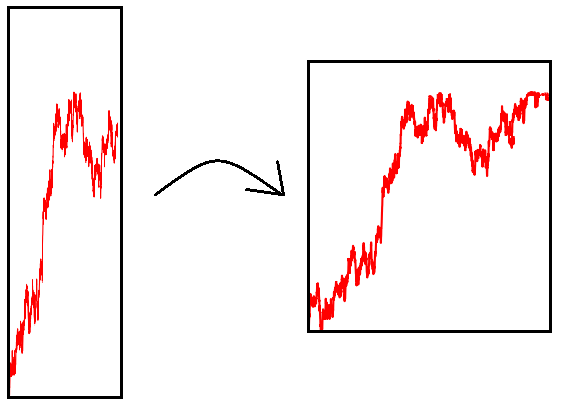
\includegraphics[width=0.8\textwidth]{pics/ch-brownian/memes-map.png}
    \caption{Example of the self-affine map used here}
    \label{fig:rectangles-graph}
\end{figure}

We wish to study the image of $G_X^{I_i}$ under these maps so identify $T_i(G_X^{I_i})=G_{X_i}^{[0,1]}$ where $X_i$ is the distribution of the new graph. Due to the scaling behaviour of $\alpha$-stable processes, 
\[
X(t) = \frac{X(R_i\, t)}{R_i^{1/\alpha}} = X_i(t)
\]
in distribution and so all the variables $X_i$ are independent $\alpha$-stable L\'evy processes with the same, original distribution $X$. Geometrically we are mapping tall, thin rectangles to the unit square which is why this scaling is often called self-affinity, see Figure \ref{fig:rectangles-graph} for an illustration. 

Let $n_i$ be any sequence of increasing, positive integers such that $\lim_{i\to\infty} n_i=\infty$. Denote by $A_i$ the event $`N_{n_i}^{1 \times 1 }((0,0),G_{X_i}^{[0,1]})=n_i^2 $'. According to the discussions above, as $X_i$ is equal to $X$ in distribution, we see that the probability of $A_i$ is $P(n_i)$ and so it exists and is strictly positive for each $i$. Figure \ref{fig:example-rectangle1} displays such an example event. 

\begin{figure}[h]\label{fig:example-rectangle1}
    \centering
    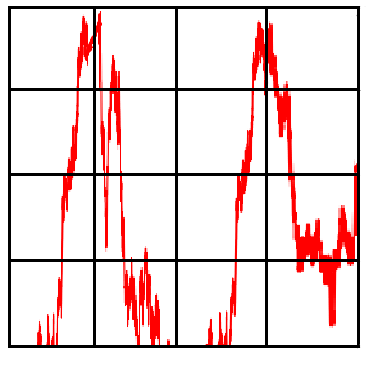
\includegraphics[width=0.6\textwidth]{pics/ch-brownian/event-rectangles.png}
    \caption{Example event satisfying the above conditions}
    \label{fig:example-rectangle1}
\end{figure}

We can choose $n_i$ to grow slowly enough such that $\sum_{i}P(n_i)=\infty$, for instance by repeating $n_i$ as many times as desired for any given $i$. Note that the $I_i$ can be chosen so that each square is disjoint and as L\'evy processes are Markov, the events $A_i$ are all independent. Then by the (second) Borel-Cantelli lemma we see that with probability $1$, infinitely many events $A_i$ occur. Now if $A_i$ happens, then
\[
N_{n_i}^{1 \times 1 }\left((0,0),G_{X_i}^{[0,1]}\right)=n_i^2.
\]
Applying the function $T^{-1}_i$ to the graph, we see that
\[
N_{n_i}^{R_i \times R_i^{1/\alpha} }\left((a_i,X(a_i)),G_{X}^{I_i}\right)=n_i^2.
\]
Note this last line tells us the number of rectangles, not squares, of side lengths $R_i / n_i$ by $R_i^{1/\alpha} / n_i$ required to cover $G_X^{[0,1]}$ inside the rectangle $[a_i, a_i + R_i] \times [X(a_i), X(a_i) + R_i^{1/\alpha}]$. 

Recall $\alpha \ge 1$ so $R_i\leq R_i^{1/\alpha}$ and all of these rectangles are taller than they are wide. When dividing each of these covering rectangles into squares of side lengths $R_i / n_i$ we see that they must be placed vertically above one another, rather than horizontally and so each of the squares must also intersect the graph as the process is right continuous and we include the lines $J$. Thus a cover of the graph inside the rectangle $[a_i, a_i + R_i] \times [X(a_i), X(a_i) + R_i^{1/\alpha}]$ by squares of side lengths $R_i / n_i$ requires all possible squares.

Hence, when restricting attention to the square $[a_i, a_i + R_i] \times [X(a_i), X(a_i)+R_i]$ and considering the covering number by squares of side lengths $R_i/n_i$ we see
\[
N_{n_i}^{R_i \times R_i }\left((a_i,X(a_i)),G_{X}^{I_i}\right)=n_i^2.
\]

As infinitely many events $A_i$ occur, using Proposition \ref{graph}, we see that almost surely
\[
\Assouad G_{X}^{[0,1]}=2.
\]


For the lower dimension we start by modifying our events. Previously, the desired outcome was that all possible squares were needed in the cover, now we ask that only the middle column intersect the graph. That is, for $n\in \mathbb{N}$,
$$G_{X}^{[0,1]} \cap (0,1]^2 \subseteq \left[\frac{\lfloor n/2 \rfloor}{n} ,  \frac{\lfloor n/2 \rfloor + 1}{n} \right] \times [0,1]$$
and $N_{n}^{1\times 1}((0,0),G_X^{[0,1]}) = n + 1$. We recall the discussion in the previous section as to why the middle column is taken here. One could ask for even less intersection, however this method suffices and is more geometrically clear, see Figure \ref{fig:rectangles-graph2}. As before, this event is measurable and has positive probability given our assumptions.

\begin{figure}[h]
    \centering
    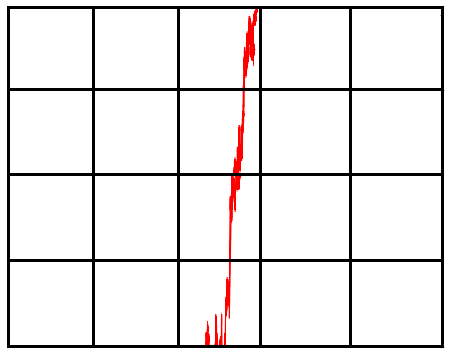
\includegraphics[width=0.6\textwidth]{pics/ch-brownian/rectangles-graph2.png}
    \caption{Example event satisfying the conditions for the lower dimension}
    \label{fig:rectangles-graph2}
\end{figure}


We then proceed in the same way: partition the graph into countably many parts $\left\{I_i \right\}$ of lengths $R_i$ and note that the images of the graph under the transformations $T_i$ still have underlying distribution $X_i =^d X$ as $X$ is $\alpha$-stable. By choosing a sequence of $n_i$ (of increasing, positive integers) correctly we will have $\sum_{i}P(n_i) = \infty$ and can denote $A_i$ the event 
$$G_{X_i}^{[0,1]} \cap (0,1]^2 \subseteq \left[\frac{\lfloor n_i/2 \rfloor}{n_i} ,  \frac{\lfloor n_i/2 \rfloor + 1}{n_i} \right] \times [0,1]$$
and $N_{n_i}^{1\times 1}((0,0),G_{X_i}^{[0,1]}) = n_i + 1$'. Since the intervals $I_i$ are disjoint, by the Borel-Cantelli lemma, with probability one, infinitely many of the above events must happen.

Thus 
\[
N_{n_i}^{R_i \times R_i^{1/\alpha}}\left((a_i,X(a_i)), G_X^{I_i}\right) = n_i + 1
\]
happens infinitely often and this intersection includes the whole `middle' column. In particular these middle $n_i$ rectangles are all in one column, so a cover by squares of the intersection of $G_X^{I_i}$ with this column will only need one column of squares. Hence, restricting to the square of side length $R_i$ gives
\[
N_{n_i}^{R_i \times R_i}\left((a_i,X(a_i)), G_X^{I_i}\right) = n_i + 1,
\]
again with the `middle' column being fully intersected. Combined with Proposition \ref{graph-lower} this completes the proof that with probability one 
\[
\lowerdim G_X^{[0,1]} = 1.
\]



\subsection{Graphs of some stochastic integrals}


	Given a function $f$ which is zero at most only finitely often and is $C^2$ on some interval, say $I'$, we can simply focus on the function restricted to $I'$, normalising to obtain a function which is $C^2$ and zero only finitely often on the unit interval. We may then assume that $f(t)>1$ for $t\in [0,1]$ by again restricting our function to an interval where the function is bounded away from zero and normalising. This is possible as the Assouad dimension is a local notion so if the dimension of some subset is full for the Assouad dimension then the whole graph will also have full dimension. Thus we assume for the rest of this proof that $f$ is a $C^2$ function which is greater than $1$.
	
	Ideally we would wish to integrate by parts in the standard Riemann–-Stieltjes sense
	\begin{equation}
	    \int_{0}^{t}f(x)dW(x)=f(t)W(t)-\int_{0}^{t}W(x)f'(x)dx.\label{eq:int-by-parts}
	\end{equation}
	The problem is that the integral on the left side of the above equation is interpreted as the It\^{o} integral, for which regular integration by parts does not hold. There is however a generalisation of this formula for stochastic integrals which holds as $f$ and $W$ are both semimartingales, see \cite{protter}[Chapter 2 Section 6] for further details. To be precise we should write the following equation
	\[
	\int_{0}^{t}f(x)dW(x)=f(t)W(t)-\int_{0}^{t}W(x)f'(x)dx-[f,W]_t.
	\]
	Here $[f,W]_t$ is the quadratic covariation between $f$ and $W$ which is defined as follows. Let $0=t_1<t_2<\dots<t_n=t$ be a partition $\mathcal{P}$ of $[0,t]$ and $\mathcal{P}_{\max}$ be the maximum of $t_{k+1}-t_k$ over all $k\in\{0,\dots,n-1\}$, then
	\[
	[f,W]_t=\lim_{\mathcal{P}_{\max}\rightarrow 0} \sum_{i=1}^{n-1} (f(t_{i+1})-f(t_{i}))(W(t_{i+1})-W(t_i)).
	\]
	The above convergence is taken in the sense of probability. By using Cauchy-Schwarz we see that:
	\[
	[f,W]_t\leq [f,f]^{1/2}_t[W,W]^{1/2}_t.
	\]
	However, it is standard that $[f,f]_t=0$ and $[W,W]_t=t$ as $f$ is $C^1$ and $W$ is the Wiener process. So we see that the integral by parts formula \eqref{eq:int-by-parts} is indeed correct for this situation. 
	
	The integral 
	\[
	\int_0^{t} W(x)f'(x)dx
	\]
	is defined to be a random process whose sample space is that of the Wiener process, where fixing a sample path of the Wiener process will determine the integral. We are interested in almost sure properties of this process and will do so by considering almost sure properties of the Wiener process.
	
	The strategy for the rest of this proof is to carefully choose a path of the Wiener process whose graph has full Assouad dimension using the previous section and then note that such a path is typical. We denote the sample space of the Wiener process as $\Omega$ and for any $\omega \in \Omega$ write $W(t,\omega)$ for the realisation of the Wiener process with respect to $\omega$.
	
	For any fixed path $\omega$, using the above discussion, we see that
	\begin{align*}
		\bigg\vert B_f\bigg(a_i+&(k+1)\frac{R_i}{n_i},\omega\bigg)-B_f\left(a_i+k\frac{R_i}{n_i},\omega\right)\bigg\vert\\
		&= \left| \int_{a_i+k\frac{R_i}{n_i}}^{a_i+(k+1)\frac{R_i}{n_i}} f(x)W(dx)\right|\\
		&= \left| f\left(x\right)W(x,\omega)\bigg\vert_{x=a_i+k\frac{R_i}{n_i}}^{a_i+(k+1)\frac{R_i}{n_i}} - \int_{a_i+k\frac{R_i}{n_i}}^{a_i+(k+1)\frac{R_i}{n_i}} W(x)f'(x)dx \right|,
	\end{align*}
	where $\lvert \cdot \rvert$ denotes the absolute value in this section.
	
	We wish to bound the above. First, we see that for almost all $\omega\in\Omega$, $W(t,\omega)$ is continuous in $t$, and therefore there is a constant $C_\omega$ such that
	\begin{equation}
	    |W(t,\omega)|\leq C_\omega \label{first-equa}
	\end{equation}
	for all $t\in [0,1]$. 
	
	The second almost sure property is described in the proof of Theorem \ref{Main}, that there are infinitely many intervals $I_i=[a_i,b_i]\subset [0,1]$ of lengths $R_i$ and a sequence $n_i\to\infty$ such that for all $k\in\{0,1,\dots,n_i-1\}$
	
	\begin{equation}
	    \left|W\left(a_i+(k+1)\frac{R_i}{n_i},\omega\right)-W\left(a_i+k\frac{R_i}{n_i},\omega\right)\right|\geq R_i^{1/2}\geq R_i. \label{ch:brownian:second-equa}
	\end{equation}
	This essentially follows from $N_{n_i}^{R_i \times R_i^{1/2}}((a_i,W(a_i), G_W^{I_i})  = n_i^2$ and recalling that the Wiener process is $2$-stable.
	
	In the following discussion we shall fix a typical $\omega$ such that $W(t,\omega)$ satisfies the above two almost sure properties, in particular, we think of $C_\omega>0$ as a fixed constant. 
	
	Since $f$ is $C^2$, we see that there is a constant $C_f$ (which does not depend on $i$) such that for all $x\in \left[{a_i+k\frac{R_i}{n_i}},{a_i+(k+1)\frac{R_i}{n_i}}\right]$, combined with equation \eqref{first-equa}, we have
	\begin{equation}
	\lvert W(x)f'(x)\rvert \leq C_f C_\omega. \label{ch:brownian:third-equa}
	\end{equation}
	
	Then using equation \eqref{ch:brownian:second-equa} the following inequality holds
	\begin{equation}
	\left| f\left(a_i+k\frac{R_i}{n_i}\right)W(x,\omega)\bigg\vert_{x=a_i+k\frac{R_i}{n_i}}^{a_i+(k+1)\frac{R_i}{n_i}} \right| \geq \left| f\left(a_i+k\frac{R_i}{n_i}\right) \right| R_i^{1/2}\geq R_i^{1/2}\label{ch:brownian:ineq-one}    
	\end{equation}
	and by equation \eqref{ch:brownian:third-equa}
	\[
	\left\vert\int_{a_i+k\frac{R_i}{n_i}}^{a_i+(k+1)\frac{R_i}{n_i}} W(x)f'(x)dx \right\vert\leq C_fC_\omega\frac{R_i}{n_i}.
	\]
	
	Since $R_i\to 0$, for all $i$ large enough we can use Taylor's theorem recalling $f$ has a continuous second derivative which yields a constant $C'$ which depends only on $f$ and $\omega$ such that
	
	\begin{align}\label{ch:brownian:main-equa}
	    \bigg\vert B_f&\bigg(a_i+(k+1)\frac{R_i}{n_i},\omega\bigg)-B_f\left(a_i+k\frac{R_i}{n_i},\omega\right)\bigg\vert \\
	    &\ge \bigg\vert f\left(a_i + k \frac{R_i}{n_i}\right) W(x,\omega) \bigg\vert_{x=a_i+k\frac{R_i}{n_i}}^{a_i+(k+1)\frac{R_i}{n_i}} + f'\left(a_i + k\frac{R_i}{n_i}\right) \frac{R_i}{n_i} W\left(a_i +(k+1) \frac{R_i}{n_i},\omega\right) \nonumber\\ 
	    &\qquad \qquad- \int_{a_i+k \frac{R_i}{n_i}}^{a_i+(k+1)\frac{R_i}{n_1}}W(x)f'(x)dx \bigg\vert  \nonumber \\
	    & \ge C'R_i. \nonumber
	\end{align}
	The above inequality holds for all $k\in\{0,\dots,n_i-1\}$. 
	
	Thus, as in the L\'evy process setting, there exists infinitely many times where the graph will fluctuate more than $R_i$ within an interval of length $R_i/n_i$. Moreover, it was previously shown that $W$ has a `zigzag' property. That is, for even integers $k$, we have
	\[
	W\left(a_i+(k+1)\frac{R_i}{n_i},\omega\right)-W\left(a_i+k\frac{R_i}{n_i},\omega\right)>0,
	\] 
	and for odd integers $k$ we have
	\[
	W\left(a_i+(k+1)\frac{R_i}{n_i},\omega\right)-W\left(a_i+k\frac{R_i}{n_i},\omega\right)<0.
	\]  
	Heuristically this says that the process increases on the first interval, decreases on the second and so forth, zigzagging from top to bottom. We can see that the expression inside the absolute values in \eqref{ch:brownian:main-equa} also satisfies a similar `zigzag' property given that $f$ is strictly positive. Therefore there is a constant $A=A(\omega,f)>0$ such that
	\[
	N_{n_i}^{R_i\times R_i} \left( (a_i, B_f(a_i)), G_{B_f}^{I_i} \right) \ge  A n_i^2
	\] 
	for infinitely many $i$. Due to the choice of $\omega$, this concludes the proof because the above argument holds for a set of full probability $\omega\in\Omega$.





\subsection{A remark on higher dimensional Brownian motion}\label{ch-brownian:sec:higher-dim}

The covering number results of Section \ref{ch:brownian:graph-proof} have natural generalisations in $\mathbb{R}^d$. Let $R_1,\dots,R_d>0$ be positive numbers and $n\in \mathbb{N}$. Given a point $\mathbf{a}\in\mathbb{R}^d$, we define $W_{n}^{R_1\times\dots\times R_d}(\mathbf{a})$ as the following collection of sets:
\begin{eqnarray*}
	\Bigg\{D_{i_1,\dots,i_d}+\mathbf{a} \, \vert \, D_{i_1,\dots,i_d}=\left[\frac{i_1}{n}R_1,\frac{i_1+1}{n}R_1\right]\times\dots\times \left[\frac{i_d}{n}R_d,\frac{i_d+1}{n}R_d\right],\\ i_j\in\{0,\dots,n-1\}, j\in\{1,\dots,d\}\Bigg\}.
\end{eqnarray*}
We see that $W_{n}^{R_1\times\dots\times R_d}(\mathbf{a})$ is a collection of rectangles with disjoint interiors. A function $f$ which intersects a full collection of $W_{n}^{R_1\times\dots\times R_d}(\mathbf{a})$ infinitely many times will have full Assouad dimension. This follows from the definitions of dimensions.

Using a similar argument as the one in Section \ref{LP}, it can be shown that this full intersection of a function and $W_{n}^{R_1\times\dots\times R_d}(\mathbf{a})$ can occur with positive probability and again by Borel-Cantelli, we obtain infinitely many occurrences almost surely. Hence the Assouad dimension of $d$-dimensional Brownian motion should be $d$. 















\section{Pushforwards of measures onto graphs of Brownian motion}


We now turn our attention to pushforwards of measures onto graphs of L\'evy processes.


Recall the definition of the graph of a L\'evy process $X$ restricted to the unit interval
\[
G_X^{[0,1]} = \left\{ (t,X(t)) \colon t \in [0,1] \right\}.
\]
There is a naturally associated function $f: [0,1] \rightarrow \mathbb{R}^2$ which maps the unit interval to the graph of the process, that is $f\colon t \mapsto (t,X(t))$. We bring attention to this function now as it will be the map we wish to use to construct pushforward measures, and for the rest of this chapter $f$ should be assumed to be this map. 





This leads us to the question of this section: given a doubling measure $\mu$ on the unit interval, is $f_*\mu$ also doubling? A similar question can be posed for uniformly perfect measures. So far we have shown the Assouad dimension of $G_X^{[0,1]}$ is almost surely 2 so there must exist at least one doubling measure on the graph. However, most measures on the graph might not even be doubling. For the Hausdorff dimension, the proof by Taylor shows that the Hausdorff dimension of the pushforward of Lebesgue measure almost surely attains the dimension of the graph itself. It turns out that this is usually not the case for the regularity dimensions.

\begin{theorem}\label{brownianthm}
	Let $\mu$ be a doubling measure on $[0,1]$ and $X$ a stable L\'evy process with the distribution $X(1)$ being non vanishing on $\mathbb{R}$. Then $f_*\mu$ is almost surely not doubling on $G_X^{[0,1]}$. Also, $f_*\mu$ is almost surely not uniformly perfect.
\end{theorem}


Trivially this implies the upper regularity dimension of $f_*\mu$ is almost surely infinity and the lower regularity dimension is almost surely zero. Therefore any measure whose upper regularity dimension approximates the dimension of the graph is highly dependent on the specific graph and so there is no one measure that attains the dimension for typical realisations, unlike the Hausdorff case. 

The following proof of this theorem is inspired by the ideas used to prove Theorem \ref{Main} however an extra case must be considered for when $\alpha < 1$. It is perhaps interesting to note we obtain a result for $\alpha < 1$ in the measure theoretic case but not the set analogue. This is simply due to the techniques used in the proofs, this second technique will be more robust to $\alpha < 1$ causing rectangles to be wide rather than tall. This result, in a way, does indicate that the Assouad dimension of the graph of a L\'evy process with $\alpha < 1$ should also be full.


\begin{proof}[Proof of Theorem \ref{brownianthm}]



Choose a L\'evy process $X$ satisfying the conditions in Theorem \ref{brownianthm} which is $\alpha$-stable and fix the graph $G_X^{[0,1]}$ realised by this process. Start by assuming $\alpha \ge 1$, the proof will work in the same way for $\alpha < 1$ given a slight modification which will be commented on later in the proof. $\mu$ is taken to be a doubling measure on the unit interval. Recall $f$ is defined to be the function which maps the unit interval to the graph of our L\'evy process and $f_*\mu$ is the pushforward measure of $\mu$ onto the graph that we wish to study.

We start by calculating the almost sure upper regularity dimension of $f_*\mu$. Let $s>0$. The general strategy for this proof is to find a sequence of events that are all independent and have positive probability. Then a simple application of the Borel-Cantelli lemma will yield that almost surely these events will happen infinitely often. By choosing our events carefully this will yield a sequence of balls that show the upper regularity dimension of the pushforward measure must be greater than $s$. As $s$ is arbitrary, this will conclude the proof.

Given our $\alpha$-scaling L\'evy process, we define the rectangle centered at $a\in [0,1]$ with side lengths $R_1,R_2$ by $Rec(a,R_1,R_2) = I(a,R_1) \times I(X(a),R_2)$ where $I(b,R) = [b-R/2,b+R/2]$ is just an interval of length $R$ and centre $b$. 

The particular events $E_i$ we are interested in are defined as follows: let $x_i \in [0,1]$, $R_i > r_i> 0$ and $\beta > 1$, then $E_i$ is the event in which $G_X^{I(x_i,R_i^{\alpha})} \subset Rec(x_i,R_i^{\alpha},R_i)$ and $Rec(x_i, r_i, r_i^{1/\alpha}) \cap G_X^{I(x_i,r_i)} = G_X^{I(x_i,r_i^{\beta})}$. These events are chosen so that the measure on the graph will be `large' on the rectangle of small side length $R^{\alpha}$ but `small' on the rectangle of small side length $r$. Figure \ref{brownian_event} is a geometric representation of such an event.  

\begin{figure}[htbp]
	\centering
	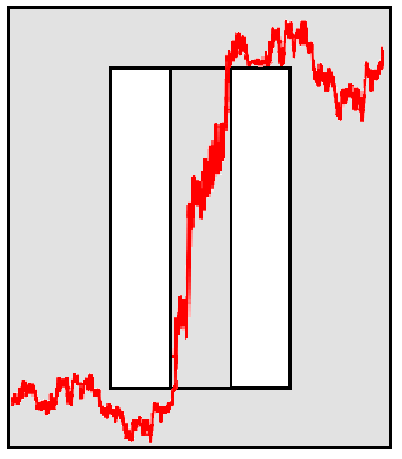
\includegraphics[width=0.4\textwidth]{pics/ch-brownian/new_rectangles.png}
	\caption{Example of an event $E_i$, the grey areas are where the graph intersects the rectangles whilst the graph will not intersect the white areas. An example of a graph satisfying this event is in red}
	\label{brownian_event}
\end{figure}

Given any sequences $x_i \in [0,1]$, $R_i > r_i > 0$ and $\beta > 1$ we can consider the associated events $E_i$ as above. To make sure the `smaller' rectangle is actually smaller, assume $R_i^{\alpha} > r_i$ without loss of generality. If $Rec(x_m,R_m^{\alpha}, R_m) \cap Rec(x_n,R_n^{\alpha},R_n) = \emptyset$ for all $m\neq n$, then the events are all independent due to the independent increment property of the L\'evy process. As long as the distribution of $X(1)$ is non-vanishing on the unit interval, the probability of any of these events is positive.

We can now choose our sequence of events. Start by picking any disjoint and strictly increasing sequence of reals  $x_i$, $\left\{1-2^{-i} \right\}_{\mathbb{N}}$ would suffice. Then the $R_i$ are taken so that the intervals $I(x_i, R_i)$ do not overlap ensuring independence, say $4^{-i}$. Initially any sequence of $r_i$ can be chosen as long as $R_i/r_i \rightarrow \infty$ and, again, $R_i^{\alpha} > r_i$ for each $i$. $\beta$ will be fixed later, for now it is just a real greater than 1. As the process is $\alpha$-stable one can map $Rec(x_i,R_i^{\alpha},R_i)$ onto the unit square via an affine map $T$ and the image of the graph under this transformation, denoted $G_{X_i}^{[0,1]}$, will have distribution $X_i$ equal to the original distribution $X(t)$ as it is scaled following the definition of $\alpha$-scaling, so $X(t) = X(R_i^\alpha t)/R_i = X_i(t)$ in distribution. This is the same process as in the proof of Theorem \ref{Main}. Therefore the probability of an event $E_i$ is equal to the probability the graph of $X_i$ stays in the unit square and 
$$Rec(1/2,r_i/R_i^{\alpha} ,r_i^{1/\alpha}/R_i ) \cap G_{X_i}^{I(1/2, r_i/R_i^{\alpha})} = G_{X_i}^{I(1/2, r_i^{\beta}/R_i^{\alpha})}.$$

Thus the probability of $E_i$ depends solely on the ratio $R_i/r_i = q_i$. If $\sum P(E_i)$ diverges then the conditions for Borel-Cantelli are satisfied and the argument continues. However, if not, the sequence $r_i$ is modified in the following way. Each $i$ gives us a ratio $q_i$ and a probability $P(E_i)$. Construct a function $g \colon \mathbb{N} \rightarrow \mathbb{N}$ such that $g(n) = \lceil \frac{1}{nP(E_n)}\rceil$ for all $n\in \mathbb{N}$. Then, keeping $R_i$ fixed, change the $r_i$ so that each ratio $q_i$ is repeated $g(i)$ many times. For instance, if $g(1) = 3$ then $r_1,r_2$ and $r_3$ are chosen so that $R_1/r_1, R_2/r_2$ and $R_3/r_3$ all give the same $P(E_1)$ and $r_4$ then is chosen with respect to $P(E_2)$ etc. The new sequence is constructed such that $\sum P(E_i)$ diverges, satisfying the conditions for Borel-Cantelli.

Hence, by the Borel-Cantelli lemma, infinitely many $E_i$ occur with probability one. So there are sequences $x_i \in [0,1]$, $R_i > r_i > 0$ and $\beta > 1$ such that, with full probability, all of the events $E_i$ happen and $R_i/r_i \rightarrow \infty$. 

Given a specific event $E_i$ we wish to consider the measure of the rectangles. The ratio of measures of such rectangles is determined by the original measure on the interval. We let $t = \lrdim \mu / 2$, this is just to have a number for which the following bound holds but is also fixed and positive due to Proposition \ref{ch-quantifying:result-heinonen} from the previous chapter. Thus we obtain the following bound:
\[
\frac{f_*\mu(Rec(x_i,R_i^{\alpha},R_i))}{f_*\mu(Rec(x_i,r_i,r_i^{1/\alpha}))} = \frac{\mu(B(x_i, R_i^{\alpha}))}{\mu(B(x_i, r_i^{\beta}))} \ge C\left(\frac{R_i^{\alpha}}{r_i^{\beta}}\right)^t, 
\]
where $C$ comes from the definition of the lower regularity dimension.

The only variable left to be fixed is $\beta$. We wish to have the above ratio greater than $C(R_i/r_i)^s$. After a short calculation, it is clear that this is always true if $\beta \ge \alpha + s/t$. Thus by choosing such a $\beta$ we have
\[
\frac{f_*\mu(Rec(x_i,R_i^{\alpha},R_i))}{f_*\mu(Rec(x_i,r_i,r_i^{1/\alpha}))} \ge C\left(\frac{R_i^{\alpha t}}{r_i^{\alpha t + s} }\right) \ge C\left(\frac{R_i^{\alpha t + s}}{r_i^{\alpha t + s} }\right)  \ge
C\left(\frac{R_i}{r_i}\right)^s. 
\]

To show the upper regularity dimension is greater than $s$ we need to consider balls not rectangles. Thankfully due to our construction $B(x_i,R_i) \supset Rec(x_i, R_i^\alpha, R_i)$ and $B(x_i,r_i) \subseteq Rec(x_i, r_i, r_i^{1/\alpha})$. Hence
\[
\frac{f_*\mu(B(x_i,R_i))}{f_*\mu(B(x_i,r_i))} \ge \frac{f_*\mu(Rec(x_i,R_i^{\alpha},R_i))}{f_*\mu(Rec(x_i,r_i,r_i^{1/\alpha}))} \ge C\left(\frac{R_i}{r_i}\right)^s ,
\]
completing the proof.

When $\alpha < 1$ much of the above argument still holds, that is we can construct the same events $E_i$ and due to the distribution of $X(1)$ they will have positive probability. Since the process is stable we can choose an infinite sequence of events such that the sum of the probabilities is infinite and then Borel-Cantelli says that infinitely many must occur with probability one. Note however that the rectangle $Rec(x_i, R_i^{\alpha}, R_i)$, for suitable variables, is now wider than it is tall. Therefore the final step where we switch back from rectangles to balls needs to be modified and a different $\beta$ must be chosen. We assume the same set-up has been followed as the $\alpha \ge 1$ case and arrive at
\[
\frac{f_*\mu(Rec(x_i,R_i^{\alpha}, R_i))}{f_*\mu(Rec(x_i,r_i, r_i^{1/\alpha}))} \ge C \left( \frac{R_i^{\alpha}}{r_i^{\beta}} \right) ^t.
\]
The natural upper bound for this with respect to balls is 
\[
\frac{f_*\mu(B(x_i, R_i^{\alpha}))}{f_*\mu(B(x_i,r_i^{1/\alpha}))} \ge \frac{f_*\mu(Rec(x_i,R_i^{\alpha}, R_i))}{f_*\mu(Rec(x_i,r_i, r_i^{1/\alpha}))}
\]
where $R_i$ and $r_i$ must be chosen so that $r_i^{1/\alpha}  \le R_i^{\alpha}$ which follows from the previous conditions. We wish to show that 
\[
\frac{f_*\mu(B(x_i, R_i^{\alpha}))}{f_*\mu(B(x_i,r_i^{1/\alpha}))} \ge C \left( \frac{R_i^{\alpha}}{r_i^{1/\alpha}} \right)^s
\]
and by choosing $\beta \ge s/ (t\alpha)$, as long as $s \ge t$, it follows that
\[
\frac{f_*\mu(B(x_i, R_i^{\alpha}))}{f_*\mu(B(x_i,r_i^{1/\alpha}))} \ge C \left( \frac{R_i^{\alpha}}{r_i^{\beta}} \right) ^t \ge C \left(\frac{R_i^{\alpha}}{r_i^{1/\alpha}}\right)^s
\]
as desired.

For the lower regularity dimension it suffices to change the events $E_i$ in the following way. Assuming $\alpha>1$, let $x_i \in [0,1]$, $R_i > r_i > 0$ and $\beta < 1$, then $E_i$ is the event where $G_X^{I(x_i, R_i)} \cap Rec(x_i,R_i,R_i^{1/\alpha}) \subseteq Rec(x_i, r_i^{\beta}, R_i^{1/\alpha})$ and $G_X^{I(x_i, r_i)} \subseteq Rec(x_i, r_i^{\alpha}, r_i)$. The previous argument then works in much the same way, showing that the lower regularity dimension of $f_*\mu$ is zero as desired.

\begin{figure}[htbp]
	\centering
	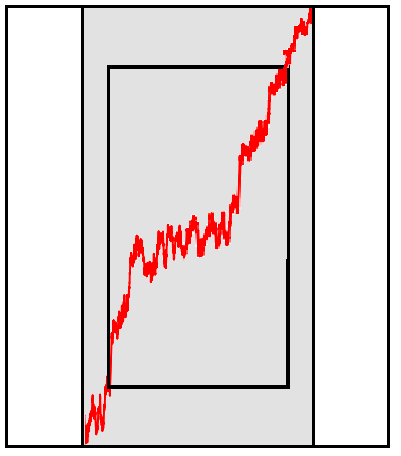
\includegraphics[width=0.4\textwidth]{pics/ch-brownian/rectangles.png}
	\caption{Example of an event $E_i$ for the lower regularity dimension, the grey areas are where the graph intersects the rectangles whilst the graph will not intersect the white areas}
	\label{brownian_event_lower}
\end{figure}


\end{proof}



